\documentclass[12pt,letterpaper]{article}
\usepackage[a4paper, top=1.2in, bottom=1.4in, left=1in, right=1in]{geometry}
\usepackage{graphicx} % Required for inserting images
\graphicspath{ {./img/} }
\usepackage[spanish]{babel}
\usepackage{float}
\usepackage{fancyhdr}
\setlength{\parskip}{1em}  % Adds space between paragraphs (1em)
\usepackage{amsmath,amssymb}
\usepackage{booktabs}
\usepackage{tikz}
\usepackage{listings}
\usepackage[utf8]{inputenc}

\usepackage{xcolor}

\lstset{
    language=Python,
    basicstyle=\ttfamily\footnotesize,
    keywordstyle=\color{blue}\bfseries,
    commentstyle=\color{gray}\itshape,
    stringstyle=\color{orange},
    showstringspaces=false,
    frame=single,
    breaklines=true
}
\usepackage{subcaption}
\newcommand{\tikzmark}[1]{\tikz[baseline,remember picture] \coordinate (#1) {};}
\usetikzlibrary{positioning}
\usetikzlibrary{shadows,arrows.meta} % For adding edges label
\usetikzlibrary{calc}
\usepackage{eso-pic}
\usepackage[backend=biber, defernumbers=true, citestyle=numeric-comp, bibstyle=ieee, sorting=none]{biblatex}
\addbibresource{bibliography/bibliography.bib}
\DeclareBibliographyCategory{cited}
\AtEveryCitekey{\addtocategory{cited}{\thefield{entrykey}}}
% Configurando BibLaTeX
\DefineBibliographyStrings{spanish}{
  url = {URL},
  andothers={et ~al\adddot}
}
\usepackage{listings}
\usepackage{xcolor}

\definecolor{codegreen}{rgb}{0,0.6,0}
\definecolor{codegray}{rgb}{0.5,0.5,0.5}
\definecolor{codepurple}{rgb}{0.58,0,0.82}
\definecolor{backcolour}{rgb}{0.95,0.95,0.92}

\lstdefinestyle{mystyle}{
    backgroundcolor=\color{backcolour},   
    commentstyle=\color{codegreen},
    keywordstyle=\color{magenta},
    numberstyle=\tiny\color{codegray},
    stringstyle=\color{codepurple},
    basicstyle=\ttfamily\footnotesize,
    breakatwhitespace=false,         
    breaklines=true,                 
    captionpos=b,                    
    keepspaces=true,                 
    numbers=left,                    
    numbersep=5pt,                  
    showspaces=false,                
    showstringspaces=false,
    showtabs=false,                  
    tabsize=2
}

\lstset{style=mystyle}

\AddToShipoutPictureBG{%
\begin{tikzpicture}[remember picture, overlay]
\node[opacity=.15, inner sep=0pt]
    at(current page.center){\includegraphics[scale=1.5]{img/logo-ugr2.png}};
\end{tikzpicture}%
}

\title{Análisis de Sentimientos}
\author{Miguel García López}
\date{Abril 2025}

\pagestyle{fancyplain}
\headheight 35pt
\lhead{Miguel García López}            
\chead{\textbf{\small Análisis de Sentimientos}}
\rhead{Minería de Medios Sociales \\ \today}
\lfoot{\scriptsize\LaTeX}
\cfoot{\small Análisis de Sentimientos}
\rfoot{\small\thepage}
\headsep 1.5em

\author{Miguel García López} % Nombre y apellidos

\date{\normalsize\today} % Incluye la fecha actual

\begin{document}
\begin{titlepage}
    \begin{figure}
        \vspace{-1.3cm}
        \begin{center}
            \includegraphics[width=0.75\textwidth]{img/UGR-Logo.png}
        \end{center}
    \end{figure}
    \vspace{1.3cm}
    \centering
    \normalfont \normalsize
    \textsc{\textbf{Minería de Medios Sociales - 2024-2025} \\\vspace{.15cm} Universidad de Granada} \\ [25pt]
    \huge Práctica de Análisis de Sentimientos - KNIME

    \normalfont \normalsize \vspace{.30cm}
    \textsc{Miguel García López}

\end{titlepage}

\tableofcontents
\listoffigures
\listoftables
\newpage

\section{Introducción}
Este documento aborda el tema del \textbf{análisis de sentimientos} y describe algunas de las técnicas utilizadas a lo largo de todo el proceso. El flujo de trabajo, o \textit{workflow}, se desarrollará utilizando el \textit{software} \textit{KNIME}, que integra una amplia variedad de herramientas específicas para este propósito, además de permitir la incorporación de \textit{plugins} adicionales si se requiere. Una de las principales ventajas de \textit{KNIME} es su enfoque visual para la construcción de procesos \textit{ETL}, lo que facilita la comprensión y el seguimiento del flujo de interacción con los datos.

Para este trabajo se requiere crear varios flujos usando \textit{Lexicons} concretos para calcular la orientación de sentimientos de una serie de \textit{reviews} de \textbf{IMDb}. Para ello se utilizaran los \textit{Lexicons}:
\begin{enumerate}
    \item \textbf{SentiWordNet 3.0}.
    \item \textbf{SenticNet 5}
    \item \textbf{Subjectivity Clues (Subjclue)}
\end{enumerate}

Además se deberá comparar los resultados obtenidos con las predicciones resultantes del uso de \textit{Lexicons}, con los resultados obtenidos de clasificadores de aprendizaje automático, como por ejemplo \textbf{SVM}, \textbf{Logistic Regression} u otros.

\section{Conjunto de datos}
Se utiliza como conjunto principal de datos el \textit{dataset} de \textbf{IMDb} (figura \ref{fig:dataset1}), el cual contiene un conjunto de reseñas etiquetadas con sentimientos negativos, positivos y neutros, así como el texto correspondiente a la reseña y su \textit{URL}. Para el trabajo concreto que se lleva a cabo en este documento, se filtran aquellas reseñas con clasificación neutra, ya que se van a evaluar solo clasificaciones binarias con el uso de \textit{Lexicons}.

\begin{figure}[htp]
    \centering
    \includegraphics[width=1\linewidth]{img/dataset1.png}
    \caption{Muestra del conjunto de datos de reseñas de \textbf{IMDb}}
    \label{fig:dataset1}
\end{figure}

\section{Lexicons}
Puede observarse el flujo completo realizado por el estudiante en la figura \ref{fig:knime_flow}. El primer nodo \texttt{csv\_reader} es el que lee el conjunto de datos. Posterior a su lectura se realiza un pre-procesamiento básico en el que se eliminan los signos de puntución, se pasa de tipo de dato \textit{string} a \textit{document} y se pasa todo el texto a minúscula. Con ello ya se tiene el texto listo para pasar al proceso de \textit{tagging}.

\begin{figure}[htp]
    \centering
    \includegraphics[width=1\linewidth]{img/knimeflow.png}
    \caption{Flujo completo de \textit{KNIME}}
    \label{fig:knime_flow}
\end{figure}


Los nodos lectores de archivos \textit{csv} debajo del lector del conjunto de datos, se encargan de cargar los \textit{Lexicons}, previamente procesados por un \textit{script} de \textit{Python} que ya los pasa a minúscula, limpia duplicados, manipula alguna palabra mal formada quitando signos como ``\_", etc. Se proporciona el código a continuación:

\begin{lstlisting}[language=Python]
    def clean_word(word):
        # Replace underscores with spaces
        word = word.replace("_", " ")
        # Remove accents
        word = unicodedata.normalize("NFD", word)
        word = word.encode("ascii", "ignore").decode("utf-8")
        # Convert to lowercase
        word = word.lower()
        return word
    
    def process_sentiwordnet_file(input_path, output_path):
        seen_words = set()
        with open(output_path, "w", newline="", encoding="utf-8") as csvfile:
            csv_writer = csv.writer(csvfile)
            csv_writer.writerow(["word", "polarity", "score"])
    
            with open(input_path, "r", encoding="utf-8") as infile:
                for line in infile:
                    if line.startswith("#") or line.strip() == "":
                        continue
    
                    parts = line.strip().split("\t")
                    if len(parts) >= 6:
                        pos, id_num, pos_score, neg_score, synset_terms, *gloss_parts = parts
                        pos_score = float(pos_score)
                        neg_score = float(neg_score)
    
                        if pos_score > 0 or neg_score > 0:
                            words = synset_terms.split()
                            for word in words:
                                word_clean = word.split("#")[0]
                                word_clean = clean_word(word_clean)
    
                                if word_clean not in seen_words:
                                    seen_words.add(word_clean)
                                    if pos_score >= neg_score:
                                        csv_writer.writerow([word_clean, "positive", pos_score])
                                    else:
                                        csv_writer.writerow([word_clean, "negative", neg_score])
    
    def process_subjclue_file(input_path, output_path):
        seen_words = set()
        with open(output_path, "w", newline="", encoding="utf-8") as csvfile:
            csv_writer = csv.writer(csvfile)
            csv_writer.writerow(["word", "polarity"])
    
            with open(input_path, "r", encoding="utf-8") as infile:
                for line in infile:
                    line = line.strip()
                    if not line:
                        continue
    
                    # Extract word and polarity from line
                    word_match = re.search(r"word1=(\w+)", line)
                    polarity_match = re.search(r"priorpolarity=(\w+)", line)
    
                    if word_match and polarity_match:
                        word = word_match.group(1)
                        polarity = polarity_match.group(1)
    
                        word_clean = clean_word(word)
    
                        if word_clean not in seen_words:
                            seen_words.add(word_clean)
                            csv_writer.writerow([word_clean, polarity])
    
    def process_senticnet_file(input_path, output_path):
        seen_words = set()
        with open(output_path, "w", newline="", encoding="utf-8") as csvfile:
            csv_writer = csv.writer(csvfile)
            csv_writer.writerow(["word", "polarity", "score"])
    
            with open(input_path, "r", encoding="utf-8") as infile:
                # Skip the header line
                header = next(infile, None)
    
                for line in infile:
                    line = line.strip()
                    if not line:
                        continue
    
                    # Use regex to split the line into parts, handling variable whitespace
                    parts = re.split(r"\s{2,}|\t+", line)
    
                    if len(parts) >= 3:
                        concept = parts[0].strip()
                        polarity = parts[1].strip().lower()
                        intensity = parts[2].strip()
    
                        # Clean the concept word
                        word_clean = clean_word(concept)
    
                        # Convert intensity to float
                        try:
                            intensity_float = float(intensity)
    
                            if word_clean not in seen_words:
                                seen_words.add(word_clean)
                                csv_writer.writerow([word_clean, polarity, intensity_float])
                        except ValueError:
                            print(f"Skipping invalid intensity value: {intensity} for word: {word_clean}")
    \end{lstlisting}

Todos los \textit{Lexicons} son filtrados y procesados por sentimiento negativo y positivo, para posteriormente utilizar el nodo \texttt{dictionary\_tagger} para relacionaer \textit{tags} de sentimiento con cada texto por ocurrencia de palabras de los \textit{Lexicons}. Después pasan por un meta-nodo (figura \ref{fig:metanode}) de procesado que se encarga de extraer un \textit{score} que representa la clasificación final del texto mediante una división de ocurrencias positivas y negativas. Posterior a todo ese flujo, se clasifica utilizando dos simples reglas: Si el \textit{score} es positivo, el texto es positivo, si es negativo el texto es negativo.

\begin{figure}[htp]
    \centering
    \includegraphics[width=1\linewidth]{img/metanode.png}
    \caption{Meta-nodo de procesamiento de los \textit{Lexicons} + \textit{dataset} para el \textit{tagging}}
    \label{fig:metanode}
\end{figure}

\subsection{Resultados}

Los resultados obtenidos por cada \textit{Lexicon} (figuras \ref{fig:cm_sentiwordnet}, \ref{fig:cm_subjclue}, \ref{fig:cm_senticnet}) son, en términos generales, decentes. Concretamente \textit{senticnet} arroja unos resultados totalmente desbalanceados, siendo capaz de identificar casi siempre los comentarios positivos, pero nunca los negativos. Esto es resultado de, seguramente, un desbalance enorme en el conjunto de términos, que lleva a predecir prácticamente siempre la clase positiva. Los otros son son mucho más equilibrados, pero siguen fallando por centenares, por lo que no son demasiado útiles.

\begin{figure}[htp]
    \centering
    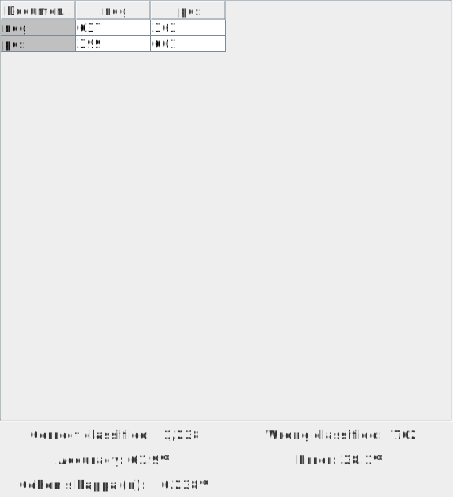
\includegraphics[width=0.4\linewidth]{img/cm_sentiwordnet.png}
    \caption{Matriz de confusión para \textit{Lexicon} de \textit{sentiwordnet}}
    \label{fig:cm_sentiwordnet}
\end{figure}

\begin{figure}[htp]
    \centering
    \includegraphics[width=0.4\linewidth]{img/cm_subjclue.png}
    \caption{Matriz de confusión para \textit{Lexicon} de \textit{subjclue}}
    \label{fig:cm_subjclue}
\end{figure}

\begin{figure}[htp]
    \centering
    \includegraphics[width=0.4\linewidth]{img/cm_senticnet.png}
    \caption{Matriz de confusión para \textit{Lexicon} de \textit{senticnet}}
    \label{fig:cm_senticnet}
\end{figure}

Se observa gráficamente en las figuras de puntos \ref{fig:scatter} las clasificaciones correspondientes a cada diccionario de términos para el conjunto de datos de reseñas.

\begin{figure}[htp]
    \centering
    \begin{minipage}{0.45\textwidth}
        \centering
        \includegraphics[width=\linewidth]{img/Senticnet - Scatter Plot.png}
        \caption{Senticnet - Scatter Plot}
    \end{minipage}
    \hfill
    \begin{minipage}{0.45\textwidth}
        \centering
        \includegraphics[width=\linewidth]{img/Sentiwordnet- Scatter Plot.png}
        \caption{Sentiwordnet - Scatter Plot}
    \end{minipage}

    \begin{minipage}{0.6\textwidth}
        \centering
        \includegraphics[width=\linewidth]{img/Subclue - Scatter Plot.png}
        \caption{Subclue - Scatter Plot}
    \end{minipage}
    \caption{Clasificación de cada \textit{Lexicon}}
    \label{fig:scatter}
\end{figure}

\section{Clasificadores ML}
Paralelo al procesamiento de los \textit{tags} se encuentra el flujo de los clasificadores de aprendizaje automático, concretamente los modelos \textbf{Support Vector Machine}, \textbf{Logistic Regression} y \textbf{Decision Tree}.

Para el uso de estos algoritmos, es necesario vectorizar los datos de forma que puedan ser usados como entrada. Se usa por este motivo el nodo \texttt{document\_vector}, el cual convierte documentos en vectores numéricos, basándose simplemente en si una palabra aparece o no (binario). Cada dimensión del vector corresponde a una palabra (o n-grama) del vocabulario.

A continuación se hace una breve descripción de cada algoritmo utilizado. Se ha probado a cambiar los hiper-parámetros de los algoritmos, pero finalmente el estudiante decidió dejar los valores por defecto.

\subsection{Support Vector Machine}
El modelo \textbf{Support Vector Machine} (SVM) busca encontrar el hiperplano que mejor separa las clases de sentimientos (por ejemplo, positivo y negativo) maximizando el margen entre ellas. En análisis de sentimientos, \textbf{SVM} es eficaz debido a su capacidad para manejar espacios de alta dimensión, como los vectores de palabras. Se ha utilizado la versión lineal del algoritmo, que es la que mejores resultados y además es la versión por defecto.

\subsection{Logistic Regression}
La \textbf{Regresión Logística} es un clasificador probabilístico que modela la probabilidad de pertenencia a una clase de sentimiento. Es ampliamente utilizado por su simplicidad, interpretabilidad y buen rendimiento en conjuntos de datos linealmente separables.

\subsection{Decision Tree}
El \textbf{Árbol de Decisión} clasifica sentimientos siguiendo una estructura jerárquica de decisiones basadas en las características del texto. Su principal ventaja en análisis de sentimientos es la facilidad para interpretar las reglas que llevan a predecir una emoción o polaridad específica.

\subsection{Resultados}

En las figuras \ref{fig:cm_lr}, \ref{fig:cm_svm} y \ref{fig:cm_dt} se pueden observar los resultados de cada algoritmo. Los tres rinden mucho mejor que la clasificación por \textit{tags} de los \textit{Lexicons}. Las predicciones del trio de clasificadores son muy balanceadas, por lo que son capaces de distinguir entre reseñas positivas y negativas sin problema alguno.

La \textit{Cohen's Kappa} es una métrica que mide el acuerdo entre dos clasificadores (o dos evaluadores) que asignan etiquetas a un conjunto de datos. Tanto \textbf{SVM} como \textbf{LR} obtiene valores para esta métrica en torno a $0.7$, lo que significa que predicen bastante bien y el acuerdo entre predicción y realidad es considerablemente mejor de lo que se lograría por azar.

El mejor modelo es el árbol de decisión, cuyo \textit{cohen's kappa} es de $0.85$ (es muy consistente) y tiene una precisión del $90\%$.

\begin{figure}[htp]
    \centering
    \includegraphics[width=0.4\linewidth]{img/cm_lr.png}
    \caption{Matriz de confusión para \textbf{Logistic Regression}}
    \label{fig:cm_lr}
\end{figure}

\begin{figure}[htp]
    \centering
    \includegraphics[width=0.4\linewidth]{img/cm_svm.png}
    \caption{Matriz de confusión para \textbf{SVM}}
    \label{fig:cm_svm}
\end{figure}

\begin{figure}[htp]
    \centering
    \includegraphics[width=0.4\linewidth]{img/cm_dt.png}
    \caption{Matriz de confusión para \textbf{Decision Tree}}
    \label{fig:cm_dt}
\end{figure}

La curva \textbf{ROC} se genera trazando la tasa de verdaderos positivos contra la tasa de falsos positivos para diferentes umbrales de decisión. El área bajo esta curva (\textbf{AUC-ROC}) es una medida de la capacidad discriminativa del modelo. Al ajustar el umbral de decisión, que por defecto suele ser $0.5$ en muchos clasificadores, se puede priorizar según las necesidades de la aplicación:

\begin{itemize}
    \item Mayor sensibilidad (\textit{recall}): reducir el número de falsos negativos.
    \item Mayor especificidad: reducir el número de falsos positivos.
\end{itemize}

En la figura \ref{fig:roc} se observan los valores de área bajo la curva \textbf{ROC} para los tres clasificadores. Los tres obtienen valores casi idénticos, por lo que se puede concluir, junto a la información previamente analizada, que separan perfectamente las clases positivas y negativas.

\begin{figure}[htp]
    \centering
    \includegraphics[width=1\linewidth]{img/roc.png}
    \caption{Visualización de curvas \textit{ROC} para los tres clasificadores}
    \label{fig:roc}
\end{figure}

\newpage

\section{Conclusión}

El análisis de sentimientos mediante diferentes técnicas ha demostrado resultados significativamente diversos. Los enfoques basados en \textit{Lexicons}, aunque conceptualmente simples, presentaron limitaciones importantes. Especialmente \textit{senticnet} mostró un sesgo notable hacia las clasificaciones positivas, mientras que las otras dos versiones ofrecieron resultados más equilibrados pero aún insuficientes para aplicaciones prácticas.

En contraste, los algoritmos de aprendizaje automático demostraron ser claramente superiores. El Árbol de Decisión destacó con una precisión del $90\%$ y un coeficiente \textit{Cohen's Kappa} de $0.85$. Las curvas \textbf{ROC} confirmaron la excelente capacidad discriminativa de estos modelos, con áreas bajo la curva prácticamente idénticas.

Este estudio evidencia que, para el análisis de sentimientos en reseñas de \textbf{IMDb}, los métodos basados en aprendizaje automático superan significativamente a los enfoques léxicos tradicionales.

\end{document}
